\chapter{Experimental evaluation}
\label{06:chapter:title}

This chapter is devoted to testing and experimentally evaluating of proposed parallel execution designed and implemented in
Chapters~\ref{04:chapter:title},~\ref{05:chapter:title}.
In addition, we designed experiments to prove the parallelism we created scales (i.e., method or class-wide).
At the same time, we calculated Amhdal's law for each experiment and compared it with the achieved result.

\section{Experiments design}

Celkový návrh experimentov sa rozlišuje do troch hlavných kategórií; (a) pre-liminary experiments, ktoré sú navrhnuté
pre dokázanie, že nami navrhnutá paralelizácia je schopná vertikálneho škálovania. Tieto experimenty budú vykonané
ako pre malé Kubernetes inštancie (i.e, Minikube) tak zároveň aj pre multi-node klastre.
Očakávané výsledky by mali byť pozitívne pretože tieto paralelizácia bude mať najlepší možný scénar vykonávania (f.e., pre method-wide paralalelizáciu
to bude testovacia trieda obsahujúca iba testy, ktoré sú schopné paralelného výpočtu, obdobne tak pre class-wide parallelizáciu.);
(b) dalšiou častou budú acceptance experimenty, ktoré budú predovšetkým mať za úlohu dodať nám informáciu, zda je efektívne
využívať paralelizáciu na pre malé inštancie Kubernetes ale zároveň tak pre veľké inštancie. Acceptance experimenty
budú zahrňovať v sebe podmnožinu našich system testov, kde sa samozrejme budú vyskytovať aj testy a testovacie triedy,
ktoré nie su schopné paralleného vykonávania a teda bude dochádzať ku synchronizácií a čakaniu. Tým pádom je možné, že
pre acceptance experimenty nebude paralelizácia vobec vhodná, pretože vačšinou sa jedná o testy kde máme v každej
testovacej triede približne jeden alebo dva testy a celková preparion fáza testovacej triedy je dlhá.; (c) posledným
typom experimentov budú tzv. regression, ktoré už budú obsahovať celú testovaciu sadu, ktorú aktuálne ponúka projekt Strimzi.
Vďaka tomu bude môct povedať, či je daná paralelizácia vhodná aj pre celkový produkt. Zároveň sa tu očakáva výrazné zrýchlenie
už len z dovodu, že sa často jedná o testovacie triedy obsahujúce 10 až viac testov. Na druhú stranu tu však máme aj veľa
testov, ktoré potrebujú na svoje vykonávanie totálnu izoláciu čo može celý výpočet spomaliť.

Pre vykonanie všetkých experimentov bude predovšetkým využívať Openstack, ktorý nám dodá potrebné HW zdroje.
Čo sa týka pre-liminárnych experimentov budeme používať 4 typy inštancií:
\begin{itemize}
    \item Kubernetes cluster \---\ multi-node, kde táto inštancia bude poskytovať 24 virtual cores a 48 GB RAM (bez počítania master nodov)
    \item Minikube \---\ single-node, kde táto inštancia bude poskytovať dve virtuáne jadrá s 8GB RAM
    \item Minikube \---\ single-node, kde táto inštancia bude poskytovať štyri virtuálne jadrá s 16GB RAM
    \item Minikube \---\ single-node, kde táto inštancia bude poskytovať osem virtuálnych jadier a 32GB RAM
\end{itemize}

\section{Preliminary experiments}

Recall~\ref{04:amdalhlaw} Amdalh's formulu z Kapitoly~\ref{03:chapter:title}.
Nato aby sme začali daný experiment nebude tentokrát počítať unit
jednotku ako počet testov ale zameriame sa na overall test execution time.
Zavedieme zároveň novú formulu (\eqref{eqn:t-new-formula}), ktorá nám zároveň vypočíta teoretický čas po zrýchlení a následne tak vďaka tomuto
výsledku vypočítame celkové možné zrýchlenie pomocou formule (\eqref{eqn:acc-formula}). Všetky značenia sú rovnaké
ako popísané v Kapitole 3 pri Amdalhovom zákone akurát tu máme \emph{T\_{new}} a \emph{T\_{old}}). \emph{T\_{old}} popisuje čas nutne vykonaný
(i.e., sekvenčne) daným taskom. Na druhú stranu \emph{T\_{new}} popisuje čas po zrýchlení (\eqref{eqn:t-new-formula}).

\begin{equation}
    \label{eqn:t-new-formula}
    T_{new} = (1 - p) * T_{old} +  \frac{p}{s} * T_{old}
    \tag{4}
\end{equation}

\begin{equation}
    \label{eqn:acc-formula}
    S = \frac{T_{old}}{T_{new}}
    \tag{5}
\end{equation}

\subsection{Method-wide}

V prípade našeho experimentu budeme mať k dispozící našu testovaciu triedu **SecurityST**, ktorá v sebe zahrňuje 21 testov.
Všetky tieto testy sa možu vykonávať parallene a tým su pre náš perfektným kandidátom, na získanie informacie že daná
paralelizácia škáluje. Čo je nutné podotknúť je fakt, že pred celkovým spusteným testov sa deployuje zdieľaný Cluster Operator,
kde vačšinou tento deployment trvá od 1m až po 6m (i.e., preto strednú hodnotu 3m). Čiže v našom prípade celková časť
ktorá sa bude dať paralelizovať bude rovná $p = \frac{171}{174} $  Prvú inštanciu ktorú použijeme bude multi-node
Kubernetes klaster s 24 virtual cores a 48 GB RAM. My zároveň vieme koľko času trvá vykonanie danej testovacej triedy
sekvenčne a túto informáciu použijeme v Amdalh's zákone.
\begin{equation}
    \label{eqn:security-st-time-ocp}
    T_{new} = (1 - \frac{171}{174}) * 174 +  \frac{ \frac{171}{174}}{24} * 174 = ~**10 minutes**
    \tag{6}
\end{equation}
Toto je teoretický čas, ku ktorému by sme sa mali blížiť v rámci testov (\eqref{eqn:security-st-time-ocp}).
Zároveň tak celkové zrýchlenie bude až 24 times. Samozrejme z praxe vieme že presne takéto zrýchlenie nedostaneme
iba sa k nemu možeme čiastoćne priblížiť.
\begin{equation}
    \label{eqn:method-wide}
    S = \frac{174}{10} =17.4x
    \tag{7}
\end{equation}
We use the following notation in the tables:
\begin{itemize}[itemsep=1mm, parsep=0pt]
    \item {\xmark} \---\ disabled parallelism (f.e., method or class-wide), or test execution containing errors
    \item {\cmark} \---\ enabled parallelism (f.e., method or class-wide), or test execution without any issues
    \item {\fontencoding{U}\fontfamily{futs}\selectfont\char 66\relax} \---\ test execution with flaky tests because of resource capacity
\end{itemize}

V nasledujúcej tabuľke~\ref{06:tab:01:securityst-ocp-multinode}, možeme vidieť jednotlivé preliminárne experimenty vykonané
nad našou implementáciou. Pre názornosť je tam zároveň obsiahnutá sekvenčná varianta. Aby sme zistili či daná parallelizácia
škáluje tam sme začali pomaly zvyšovať použité vlákna (i.e., začali sme od 2 až po 16). V rámci experimentovania sme zistili,
že najvhodnejším kandidátom pre SecurityST by bolo behať to až na 12 vláknach. Ako zároveň možeme vidieť na
tabuľke~\ref{06:tab:01:securityst-ocp-multinode} tak pri použití 16 vlákien bol daný Kubernetes cluster zneškodnený.
Dovodom bolo hlavne kapacita zdrojov (i.e., pre každý test sa deployne Kafka cluster a mnoho dalších zdrojov), a Kubernetes API.
Zároveň si možeme všimnúť, že sme nedosiahli teoretického zrýchlenia, ktoré sme vypočítali (\eqref{eqn:security-st-time-ocp}).
Toto je však podmienené viacerými faktormi (f.e., testy netrvajú rovnaký čas alebo pomalší deployment volumes v rámci Kafka clusterov).
Čo je si ale treba uvedomiť je že ak v prípade neobmedzených zdrojov (i.e., cores, RAM) by sme nemohli prekonať nami vypočítané zrýchlenie
pretože to možeme vyjadriť ako limitu (\eqref{eqn:amdalh-limit}).
\begin{table}[ht!]
    \centering
    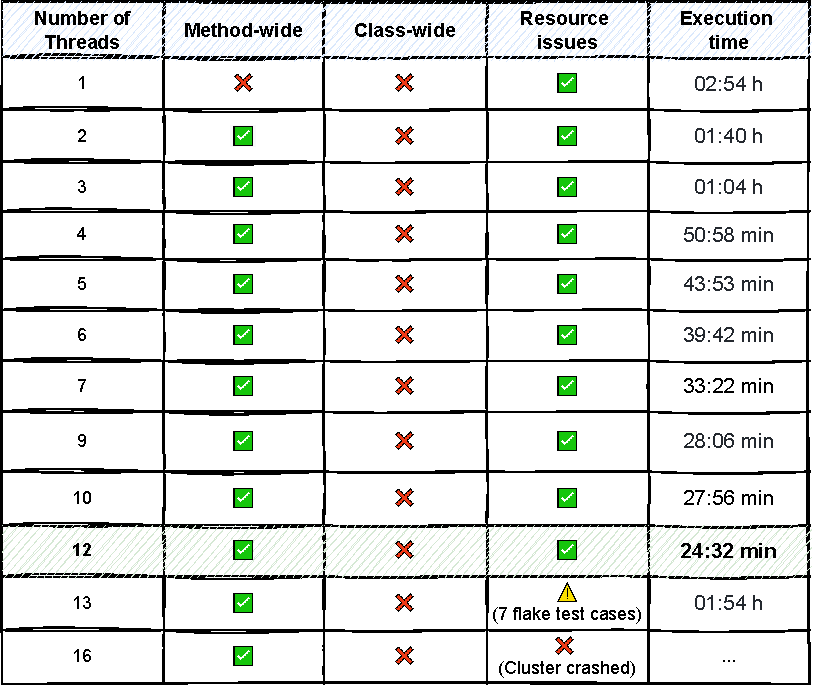
\includegraphics[scale=0.8]{obrazky-figures/08-experiments/06-exp-final-smoke-method-wide-ocp}
    \caption{Preliminary experiments with Security test suite containing twenty-one test cases, which all can be run in parallel.
    Each test case deploys Kafka cluster, which perfectly verifies if Kubernetes cluster or Minikube (i.e., single-node) can handle such a load.}
    \label{06:tab:01:securityst-ocp-multinode}
\end{table}

\begin{equation}
    \label{eqn:amdalh-limit}
    \lim_{s\to\infty} S_{max} = \frac{1}{1-p} =  \frac{1}{1-\frac{171}{174}} = 58x
    \tag{8}
\end{equation}
Naše nadobutnuté zrýchlenie v rámci perfektnom prostredí je menšie než $S_{\max} = 58x$ a zároveň tak $S_{teo} = 17.4x$.
Čo však potvrdzuje fakt, že nikdy nebudeme lepší než $S_{\max}$ a taktiež nikdy nedosiahneme možné teoretické zrýchlenie (i.e., $S_{teo}$),
pretože to je v praxi normálne. Celkovo naše zrýchlenie je rovné $S_{practical} = \frac{174}{24.5} =7.1x$, čo je veľmi skvelé.

% MINIKUBE PART
Dalšie preliminárne experimenty, ktoré sme vykonali boli na menších inštanciach kde bolo samozrejmosťou, že výsledky
zrýchlenia s porovnaním multi-node klastru budú podstatne nižšie.
Preto aj Amdalhov zákon bude obsahovať o dosť nižšie teoretické zrýchlenie. Pre mašinu obsahujúcu štyri virtuálne jadrá je
odhadujúci teoretický čas $T_{new\_teo\_medium}$, ktorý je rovný $T_{new\_teo\_medium} = (1 - \frac{182}{185}) * 185 +  \frac{ \frac{182}{185}}{4} * 185 = $ approximately 49~minutes.
A teda teoretické zrýchlenie inštancie by mohol byť $S_{new\_teo\_medium} = \frac{185}{49} = 3.8x$.
Ako však možeme vidieť na tabuľke~\ref{06:tab:01:securityst-minikube}, tak také presné zrýchlenie sme nedosiahli.
Avšak priblížili sme sa k tomu dostatočne blízko a praktické zrýchlenie je rovné $S_{new\_practical\_medium} = \frac{185}{79} = 2.34x$.
Maximálne sme mohli využiť tri jadrá, pretože v prípade štyroch jadier virtual machine padla kvoli nedostatku pamate.
CPU utilizácia bola v priebehu pri použití štyroch jadier približne na 80\%.

\begin{table}[ht!]
    \centering
    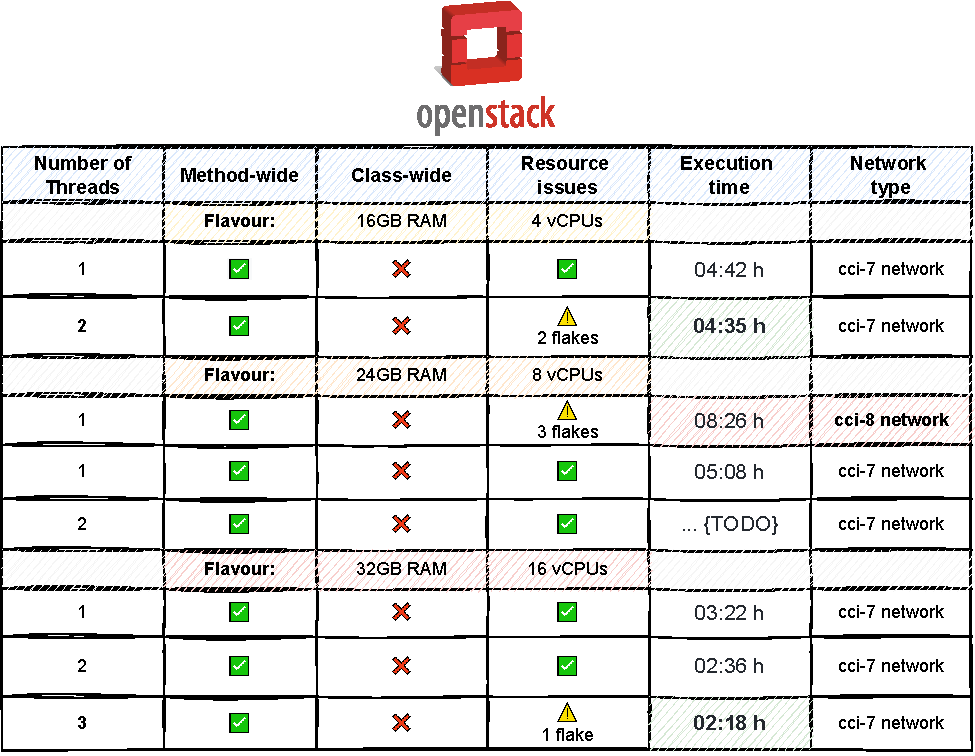
\includegraphics[scale=0.8]{obrazky-figures/08-experiments/06-exp-a-prelim}
    \caption{Preliminary experiments with Security test suite containing twenty-one test cases, which all can be run in parallel.
    Each test case deploys Kafka cluster, which perfectly verifies if Kubernetes cluster or Minikube (i.e., single-node) can handle such a load.}
    \label{06:tab:01:securityst-minikube}
\end{table}

\subsection{Class-wide}

Preliminárne experimenty pre class-wide parallezáciu sme vybrali množinu testovacích tried, ktoré podporujú túto formu
paralelizácie (i.e, @ParallelSuite).
Špecificky sa bude jednať o CruiseControlConfigurationST, HttpBridgeScramShaST, HttpBridgeCorsST, HttpBridgeKafkaExternalListenersST,
HttpBridgeTlsST, TopicST, ThrottlingQuotaST, UserST, ReconciliationST, QuotasST.

...


% b) PRELIMINARY EXPERIMENTS FOR CLASS-WIDE

\section{Acceptance experiments}

acceptance profile...

\section{Regression experiments}

regression profile...

\chapter{Future work}
\label{07:chapter:title}

\chapter{Conclusion}
\label{08:chapter:title}